% Number 962
% CAPMG NAPM  Units 
% Drag racer - CAPM and CVPM, NAPM - graphical
% JG

% Watermark
\AddToShipoutPicture*{\BackgroundPic}

\addtocounter {ProbNum} {1}

%\begin{floatingfigure}[r]{.44\textwidth}
%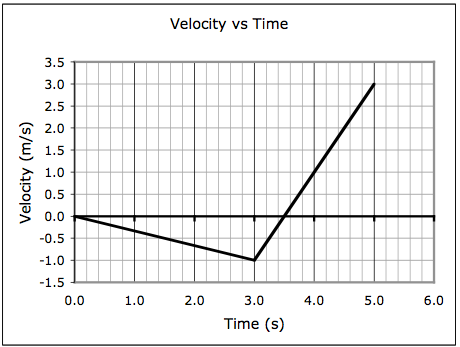
\includegraphics[scale=.54]{/Users/jgates/desktop/latex/pics/vgraph6}
%\end{floatingfigure}
 
{\bf \Large{\arabic{ProbNum}}} A drag racer begins at rest, and accelerates to ${124~\tfrac{m}{s}}$.  Once at this speed, the racer maintains it through the finish line, which is 400 meters from the start line. The car deploys a parachute after crossing the finish line.  The magnitude of the acceleration provided by the air hitting the parachute is initially ${12~\tfrac{m}{s^2}}$.
\bigskip

Assuming that this acceleration is constant, how far will the car travel after crossing the finish line but before coming to a stop? Use graphical methods.
\vfill

The acceleration depends on the speed of the car, however: the magnitude of the acceleration decreases as the car slows down.  Incorporate this idea into your analysis and come up with a new estimate of the stopping distance.  Any reasonable model consistent with what I've told you is fine.
\vfill
%\begin{center}
%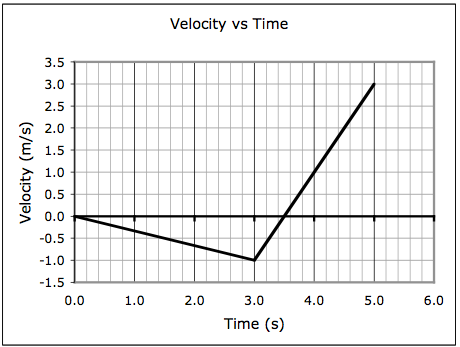
\includegraphics[scale=1]{/Users/jgates/desktop/latex/pics/vgraph6}
%\end{center}


\newpage